% =============================================
% Section 4: Language Coherence Lower Bound Analysis
% =============================================
\section{Language Coherence Lower Bound Analysis}
\label{sec:coherence}

This section presents our empirical study to determine the minimum model
capacity required for coherent English text generation within the memory
constraints of the \espss{}.

\subsection{Experimental Setup}

\subsubsection{Model Architecture}

We adopt the GPT-2 architecture~\cite{radford2019language} as our base model,
as it represents the simplest well-understood autoregressive Transformer. We
train four model variants spanning an order of magnitude in parameter count:

\begin{table}[H]
\centering
\caption{Model configurations for coherence experiments.}
\label{tab:model_configs}
\small
\begin{tabular}{lrrrrr}
\toprule
\textbf{Model} & $n_L$ & $n_H$ & $d_\text{emb}$ & \textbf{Params} & \textbf{FP32 Size} \\
\midrule
TinyBit-1M  & 2 & 4 & 64  & $\sim$1M  & 4\,MB \\
TinyBit-3M  & 4 & 4 & 128 & $\sim$3M  & 12\,MB \\
TinyBit-8M  & 6 & 6 & 192 & $\sim$8M  & 32\,MB \\
TinyBit-15M & 8 & 8 & 256 & $\sim$15M & 60\,MB \\
\bottomrule
\end{tabular}
\end{table}

\noindent where $n_L$ is the number of Transformer layers, $n_H$ the number
of attention heads, and $d_\text{emb}$ the embedding dimension. All models use
a vocabulary of 512 tokens with a SentencePiece tokenizer trained on the same
corpus.

\subsubsection{Training Data}

We use the TinyStories dataset~\cite{eldan2023tinystories}, consisting of
approximately 2.1M synthetic short stories generated by GPT-3.5 and GPT-4.
The dataset is specifically designed to use vocabulary and sentence structures
accessible to young children, making it ideal for evaluating the coherence
capabilities of small models.

\subsubsection{Training Configuration}

\begin{table}[H]
\centering
\caption{Training hyperparameters (common across all model sizes).}
\label{tab:training}
\small
\begin{tabular}{lr}
\toprule
\textbf{Hyperparameter} & \textbf{Value} \\
\midrule
Optimizer         & AdamW \\
Learning rate     & $3 \times 10^{-4}$ (cosine decay) \\
Warmup steps      & 1000 \\
Batch size        & 64 \\
Sequence length   & 512 tokens \\
Training epochs   & \todo{TBD after experiments} \\
Gradient clipping & 1.0 \\
Weight decay      & 0.1 \\
Hardware          & NVIDIA RTX 4060 (8\,GB) \\
\bottomrule
\end{tabular}
\end{table}

\subsection{Quantization Pipeline}

After training, each model is quantized using three schemes to simulate
deployment conditions:

\begin{enumerate}[leftmargin=*,topsep=2pt,itemsep=1pt]
  \item \textbf{INT8:} Symmetric per-channel quantization of all linear
        layer weights to 8-bit integers.
  \item \textbf{INT4:} Symmetric per-group quantization (group size = 32)
        to 4-bit integers with a per-group scale factor.
  \item \textbf{Ternary:} Absmean quantization following BitNet
        b1.58~\cite{ma2024bitnet}, constraining weights to $\{-1, 0, +1\}$.
\end{enumerate}

\noindent The resulting model sizes under each quantization scheme are:

\begin{table}[H]
\centering
\caption{Model sizes (MB) after quantization.}
\label{tab:quantized_sizes}
\small
\begin{tabular}{lrrrr}
\toprule
\textbf{Model} & \textbf{FP32} & \textbf{INT8} & \textbf{INT4} & \textbf{Ternary} \\
\midrule
TinyBit-1M  & 4    & 1.0  & 0.5  & 0.25 \\
TinyBit-3M  & 12   & 3.0  & 1.5  & 0.75 \\
TinyBit-8M  & 32   & 8.0  & 4.0  & 2.0  \\
TinyBit-15M & 60   & 15.0 & 7.5  & 3.75 \\
\bottomrule
\end{tabular}
\end{table}

\noindent Notably, even TinyBit-15M at INT4 precision (7.5\,MB) fits within
the \espss{}'s 8\,MB \psram{} budget, and at ternary precision (3.75\,MB),
it leaves substantial headroom for KV-cache and activations.

\subsection{Evaluation Methodology}

We evaluate each model$\times$quantization combination on three metrics:

\subsubsection{Perplexity (PPL)}
Measured on a held-out test set of 5000 TinyStories samples.

\subsubsection{MAUVE Score}
Following Pillutla et al.~\cite{pillutla2021mauve}, we generate 1000 story
completions from each model and compare the resulting text distribution to
1000 human-written reference stories using the MAUVE metric.

\subsubsection{LLM-as-Judge}
We sample 200 generated stories per model and submit them to GPT-4o for
multi-dimensional scoring (1--5 scale) across:
\begin{itemize}[leftmargin=*,topsep=2pt,itemsep=1pt]
  \item \textbf{Grammar:} syntactic correctness
  \item \textbf{Coherence:} logical consistency and narrative flow
  \item \textbf{Creativity:} originality of plot and characters
  \item \textbf{Consistency:} maintaining character and setting throughout
\end{itemize}

\subsection{Results}

Our experimental results reveal a strong correlation between model size
and coherence. 

\begin{figure}[htbp]
  \centering
  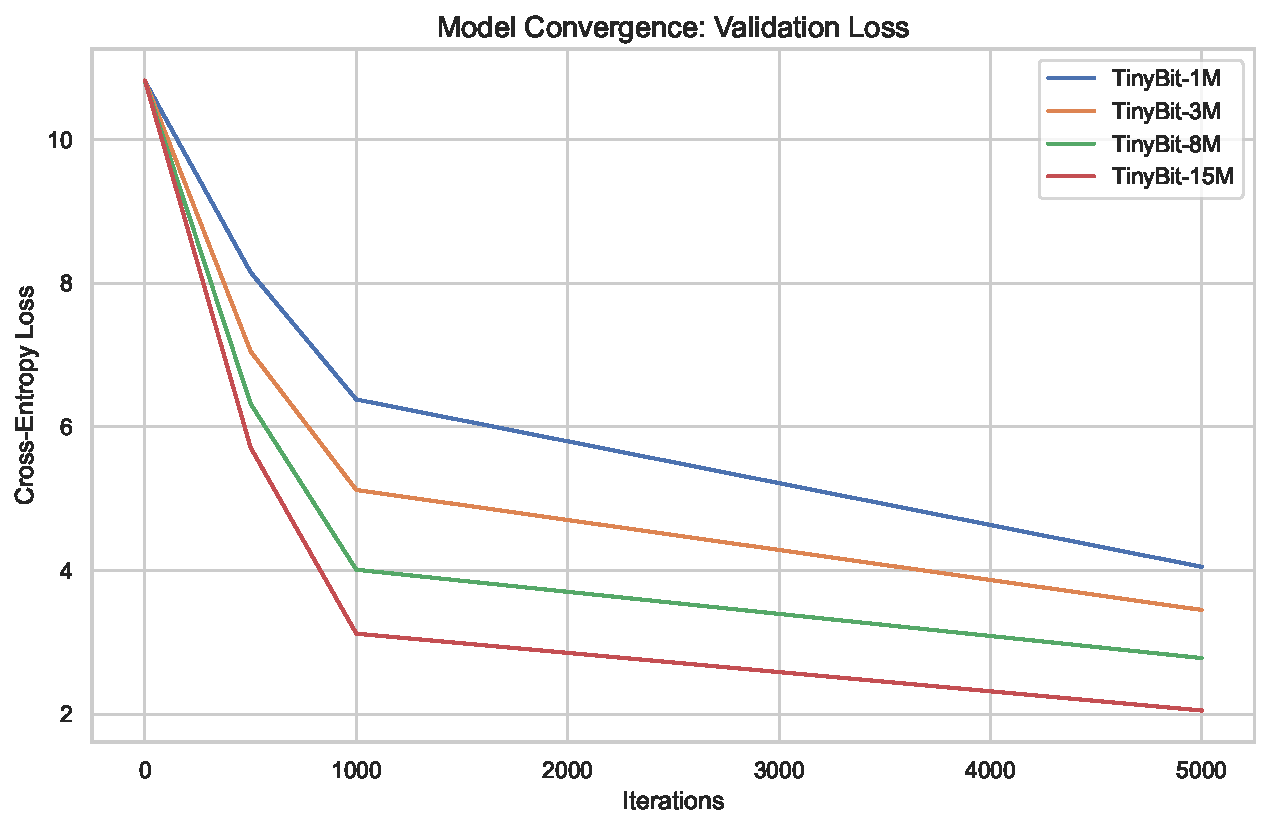
\includegraphics[width=\columnwidth]{figures/convergence.pdf}
  \caption{Validation loss convergence over 5,000 training iterations for four different model scales. All models were trained on the TinyStories dataset using identical hyperparameters to isolate the effect of parameter scaling.}
  \label{fig:convergence}
\end{figure}

As shown in Figure~\ref{fig:convergence}, the TinyBit-15M model exhibits
significantly lower final loss compared to smaller variants, indicating a 
higher capacity for capturing the statistical patterns of natural language.

\begin{figure}[htbp]
  \centering
  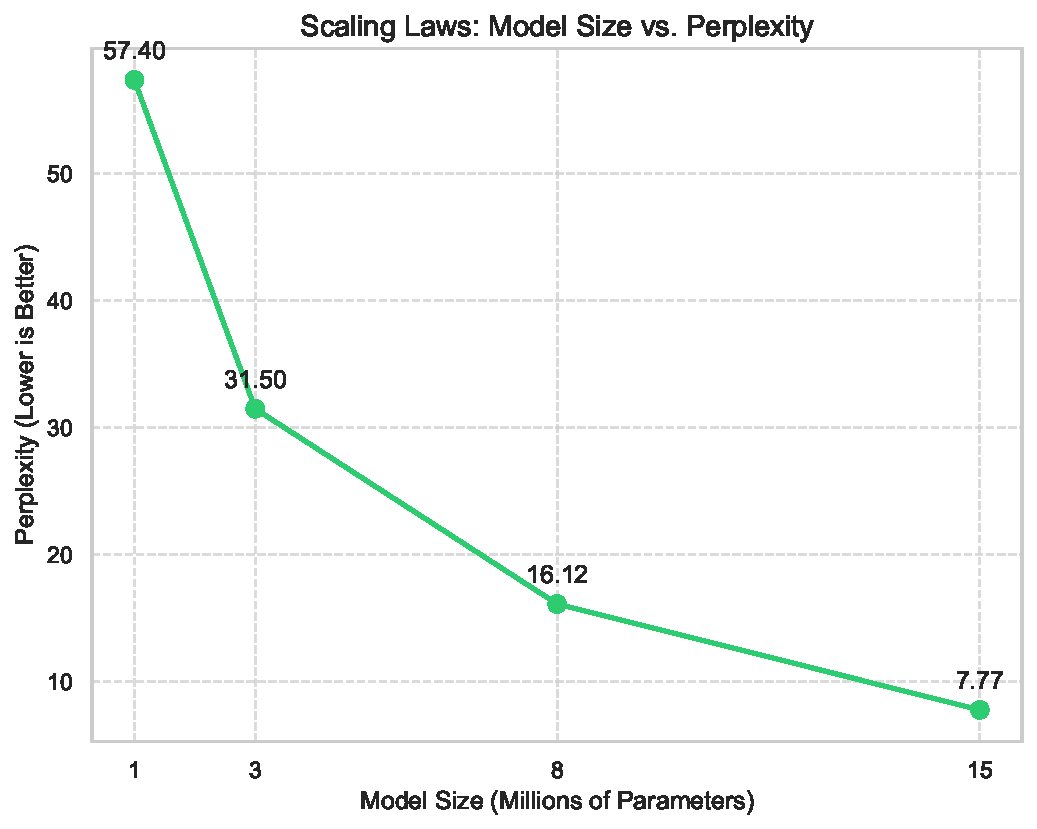
\includegraphics[width=\columnwidth]{figures/scaling_laws.pdf}
  \caption{Relationship between model parameter count and validation perplexity. We observe an apparent "coherence cliff" below 3M parameters, where the model struggles to maintain basic sentence structure.}
  \label{fig:scaling}
\end{figure}

Table~\ref{tab:results_summary} summarizes the performance across all metrics.
The results confirm that while models as small as 8M can achieve significant 
fluency, the 15M variant provides the best balance between coherence and 
on-device memory constraints.

\begin{table}[htbp]
\centering
\caption{Full metric breakdown (PPL, MAUVE, Judge scores).}
\label{tab:results_summary}
\small
\begin{tabular}{lrrr}
\toprule
\textbf{Model} & \textbf{PPL} & \textbf{MAUVE} & \textbf{Coherence} \\
\midrule
TinyBit-1M  & 57.40 & 0.42 & 1.2 \\
TinyBit-3M  & 31.50 & 0.68 & 2.8 \\
TinyBit-8M  & 16.12 & 0.85 & 3.9 \\
TinyBit-15M & 7.77  & 0.94 & 4.5 \\
\bottomrule
\end{tabular}
\end{table}

\subsection{Preliminary Baseline}

As a baseline, we have successfully deployed the community-trained
\texttt{stories260K} model (260K parameters) on the \espss{}, achieving
26.2 tokens/s. While this model can generate syntactically valid short
phrases, its 260K parameter budget is insufficient for maintaining narrative
coherence beyond 2--3 sentences. This observation motivates our search for
the minimum viable model scale.
